
\documentclass{article}

\usepackage{fancyhdr}
\usepackage{extramarks}
\usepackage{amsmath}
\usepackage{amsthm}
\usepackage{amsfonts}
\usepackage{tikz}
\usepackage[plain]{algorithm}
\usepackage{algpseudocode}
\usepackage{listings}
\usepackage{booktabs}
\usepackage{xcolor}
\usepackage[english]{babel}
\usepackage[T1]{fontenc}
\usepackage{lmodern,mathrsfs}
\usepackage{xparse}
\usepackage[inline,shortlabels]{enumitem}
\setlist{topsep=2pt,itemsep=2pt,parsep=0pt,partopsep=0pt}
\usepackage[dvipsnames]{xcolor}
\usepackage[utf8]{inputenc}
\usepackage[a4paper,top=0.5in,bottom=0.2in,left=0.5in,right=0.5in,footskip=0.3in,includefoot]{geometry}
\usepackage[most]{tcolorbox}
\tcbuselibrary{minted} % tcolorbox minted library, required to use the "minted" tcb listing engine (this library is not loaded by the option [most])
\usepackage{minted} % Allows input of raw code, such as Python code
% \usepackage[colorlinks]{hyperref}


\usetikzlibrary{automata,positioning}

\tcbset{
    pythoncodebox/.style={
        enhanced jigsaw,breakable,
        colback=gray!10,colframe=gray!20!black,
        boxrule=1pt,top=2pt,bottom=2pt,left=2pt,right=2pt,
        sharp corners,before skip=10pt,after skip=10pt,
        attach boxed title to top left,
        boxed title style={empty,
            top=0pt,bottom=0pt,left=2pt,right=2pt,
            interior code={\fill[fill=tcbcolframe] (frame.south west)
                --([yshift=-4pt]frame.north west)
                to[out=90,in=180] ([xshift=4pt]frame.north west)
                --([xshift=-8pt]frame.north east)
                to[out=0,in=180] ([xshift=16pt]frame.south east)
                --cycle;
            }
        },
        title={#1}, % Argument of pythoncodebox specifies the title
        fonttitle=\sffamily\bfseries
    },
    pythoncodebox/.default={}, % Default is No title
    %%% Starred version has no frame %%%
    pythoncodebox*/.style={
        enhanced jigsaw,breakable,
        colback=gray!10,coltitle=gray!20!black,colbacktitle=tcbcolback,
        frame hidden,
        top=2pt,bottom=2pt,left=2pt,right=2pt,
        sharp corners,before skip=10pt,after skip=10pt,
        attach boxed title to top text left={yshift=-1mm},
        boxed title style={empty,
            top=0pt,bottom=0pt,left=2pt,right=2pt,
            interior code={\fill[fill=tcbcolback] (interior.south west)
                --([yshift=-4pt]interior.north west)
                to[out=90,in=180] ([xshift=4pt]interior.north west)
                --([xshift=-8pt]interior.north east)
                to[out=0,in=180] ([xshift=16pt]interior.south east)
                --cycle;
            }
        },
        title={#1}, % Argument of pythoncodebox specifies the title
        fonttitle=\sffamily\bfseries
    },
    pythoncodebox*/.default={}, % Default is No title
}

% Custom tcolorbox for Python code (not the code itself, just the box it appears in)
\newtcolorbox{pythonbox}[1][]{pythoncodebox=#1}
\newtcolorbox{pythonbox*}[1][]{pythoncodebox*=#1} % Starred version has no frame

\tcbset{
    rcodebox/.style={
        enhanced jigsaw,breakable,
        colback=blue!5,colframe=blue!40!black,
        boxrule=1pt,top=2pt,bottom=2pt,left=2pt,right=2pt,
        sharp corners,before skip=10pt,after skip=10pt,
        attach boxed title to top left,
        boxed title style={empty,
            top=0pt,bottom=0pt,left=2pt,right=2pt,
            interior code={\fill[fill=tcbcolframe] (frame.south west)
                --([yshift=-4pt]frame.north west)
                to[out=90,in=180] ([xshift=4pt]frame.north west)
                --([xshift=-8pt]frame.north east)
                to[out=0,in=180] ([xshift=16pt]frame.south east)
                --cycle;
            }
        },
        title={#1},
        fonttitle=\sffamily\bfseries
    },
    rcodebox/.default={}, % Default title = none
    % Starred version has no frame
    rcodebox*/.style={
        enhanced jigsaw,breakable,
        colback=blue!5,coltitle=blue!40!black,colbacktitle=tcbcolback,
        frame hidden,
        top=2pt,bottom=2pt,left=2pt,right=2pt,
        sharp corners,before skip=10pt,after skip=10pt,
        attach boxed title to top text left={yshift=-1mm},
        boxed title style={empty,
            top=0pt,bottom=0pt,left=2pt,right=2pt,
            interior code={\fill[fill=tcbcolback] (interior.south west)
                --([yshift=-4pt]interior.north west)
                to[out=90,in=180] ([xshift=4pt]interior.north west)
                --([xshift=-8pt]interior.north east)
                to[out=0,in=180] ([xshift=16pt]interior.south east)
                --cycle;
            }
        },
        title={#1},
        fonttitle=\sffamily\bfseries
    },
    rcodebox*/.default={}, % Default title = none
}

% Custom tcolorbox environments
\newtcolorbox{rbox}[1][]{rcodebox=#1}
\newtcolorbox{rbox*}[1][]{rcodebox*=#1}

% Basic Document Settings
\topmargin=-0.45in
\evensidemargin=0in
\oddsidemargin=0in
\textwidth=6.5in
\textheight=9.0in
\headsep=0.25in
\linespread{1.1}

\pagestyle{fancy}
\lhead{\hmwkAuthorName}
\chead{\hmwkClass\ (\hmwkClassInstructor): \hmwkTitle}
\rhead{\firstxmark}
\lfoot{\lastxmark}
\cfoot{\thepage}
\renewcommand\headrulewidth{0.4pt}
\renewcommand\footrulewidth{0.4pt}
\setlength\parindent{0pt}

% Homework Details
\newcommand{\hmwkTitle}{Asignacion 3}
\newcommand{\hmwkDueDate}{Octubre 24, 2025}
\newcommand{\hmwkClass}{ESMA 6787}
\newcommand{\hmwkClassInstructor}{Israel Almodovar}
\newcommand{\hmwkAuthorName}{\textbf{Alejandro Ouslan}}

% Title Page
\title{
	\vspace{2in}
	\textmd{\textbf{\hmwkClass:\ \hmwkTitle}}\\
	\normalsize\vspace{0.1in}\small{Due\ on\ \hmwkDueDate}\\
	\vspace{0.1in}\large{\textit{\hmwkClassInstructor}}
	\vspace{3in}
}

\author{\hmwkAuthorName}
\date{}


% Begin document
\begin{document}
\maketitle
\pagebreak
\tableofcontents
\pagebreak

% Homework problem 1
\section{problem 1}
Define using your own words:
\begin{enumerate}
	\item Estimate $c'\beta$:
	      \[
		      \begin{split}
			      Y = X\beta + \epsilon      \\
			      \hat{beta} = (X'X)^{-1}X'Y \\
			      \hat{c'}\beta = c'\hat{beta}
		      \end{split}
	      \]
	\item Power: It's the probability of correctly rejecting the null hypothesis when the alternative is true
	\item Null hypothesis: It is the assumed reality or state of the research question
	\item Alternative hypothesis: It is the testing question of the research
	\item Test Statistics: it is the criteria for rejecting the null the hypothesis
	\item Non-centrality parameter: it quantifies how much the true value of the parameter is off by
	\item Details about the non-centrality parameter:
\end{enumerate}

\section{Problem 2}
A student commented in a discussion group: ”Random permutations are used to assign treatments
to experimental units with a randomized block design just as with a completely randomized design.
Hence, there is no basic difference between these two designs.” Comment.

\textbf{Answer:}The assignment may be the same but the structure is different given that the data is partitioned
in section or "blocks". This reduces the variance at the cost of power

\section{Problem 3}
Five treatments are studied in an experiment with a randomized complete block design using four
blocks. Obtain randomized assignments of treatments to experimental units

\textbf{Answer:}This should comprise of 4 block with 5 entities each receiving on of the treatments. All of the treatments
should be present in each block (assuming it a balance block design). This should total to 20 observations

\section{Problem 4}
Two treatments and a control are studied in an experiment with a randomized block design. Five
blocks are employed, each containing four experimental units. In each block. Each treatment is to
be assigned to one experimental unit, and the control is to be assigned to two experimental units.
Obtain randomized assignments of treatments to experimental units

\textbf{Answer:} Each block should contain 4 observations where we will assign randomly the 2 treatments
the rest of the observations should then be the controls.

\section{Problem 5}
An accounting firm, prior to introducing in the firm widespread training in statistical sampling for
auditing. Tested three training methods: (1) study at home with programmed training materials.
(2) training sessions at local offices conducted by local staff, and (3) training sessions in Chicago
conducted by national staff. Thirty auditors were grouped into 10 blocks of three. According to
time elapsed since college graduation. And the auditors in each block were randomly assigned to the
three training methods. At the end of the training, each auditor was asked to analyze a complex
case involving statistical applications; a proficiency measure based on this analysis was obtained
for each auditor. The results were (block 1 consists of auditors graduated most recently, block 10
consists of those graduated most distantly):
\begin{enumerate}
	\item Why do you think the blocking variable ”time elapsed since college graduation” was employed?

	      \textbf{Answer:} This is to control for experience as people who have spend more time since graduation
	      are more likely to have more experience and hence more likely to preform better in the tests
	\item Consider the following linear model with blocking effects.
	      $$
		      y= X_1 \theta + X_2 \tau + \epsilon
	      $$
	      Explain each of the terms carefully in context of the problem
	      \begin{enumerate}
		      \item $y$: Is the scores reported
		      \item $X_1$ is the treatment effects matrix for the training sessions
		      \item $X_2$: is the block effects matrix for the groups
		      \item $\theta$: is the treatment effect coefficient
		      \item $\tau$: is the block effects coefficient
		      \item $\epsilon$: is the error term o unobserved effects
	      \end{enumerate}
	\item Write the design matrix $X_1$.
	      $$
		      X_1 =\mathbf{1}_{10} \otimes I_3
	      $$

	\item Write the design matrix $X_2$.
	      $$
		      X_2 = I_{10} \otimes \mathbf{1}_3
	      $$
	\item obtain a estimate for the treatment effects $\hat{\tau}$.
	      $$
		      \hat{\tau} = \begin{bmatrix}
			      4.9  \\
			      15.3 \\
		      \end{bmatrix}
	      $$

	\item Obtain the analysis of variance table.
	      \[
		      \begin{array}{lrrrr}
			      \hline
			      \text{Source}   & \text{Sum of Squares (SS)} & \text{df} & F      & \text{p-value}      \\
			      \hline
			      \text{Block}    & 434.300                    & 9         & 5.9575 & 6.64 \times 10^{-4} \\
			      \text{Training} & 1220.867                   & 2         & 75.362 & 1.79 \times 10^{-9} \\
			      \text{Residual} & 145.800                    & 18        & -      & -                   \\
			      \hline
		      \end{array}
	      \]

	\item Report the value of the estimated mean square error.
	      $$
		      8.1
	      $$
	\item Test whether the mean proficiency is the same for the three training methods. Use a level of significance
	      $\alpha = 0.05$. State the alternative, decision rule, and conclusion. What is the p-value of the test?
	      $$
		      F= 75.362, \quad p-value = 1.79 \times 10^{-9}
	      $$
	\item Make all pairwise comparisons between the training method means; use the Tukey procedure with a 90\% family
	      confidence coefficient. State your findings.

	      \[
		      \begin{array}{lrrrrrr}
			      \hline
			      \text{Comparison}           & \text{Mean Difference} & p\text{-adj} & \text{Lower 90\% CI} & \text{Upper 90\% CI} & \text{Reject } H_0? \\
			      \hline
			      \text{Method 1 vs Method 2} & 4.9                    & 0.0639       & 0.458                & 9.342                & \text{Yes}          \\
			      \text{Method 1 vs Method 3} & 15.3                   & 0.0000       & 10.858               & 19.742               & \text{Yes}          \\
			      \text{Method 2 vs Method 3} & 10.4                   & 0.0001       & 5.958                & 14.842               & \text{Yes}          \\
			      \hline
		      \end{array}
	      \]

	      \textbf{Interpretation:}

	      \begin{itemize}
		      \item Training Method 3 has the highest mean proficiency and is significantly better than both Methods 1 and 2.
		      \item Training Method 2 shows a moderate improvement over Method 1, which is significant at the 90\% confidence level.
		      \item Therefore, all pairwise differences between training methods are statistically significant at the chosen family-wise confidence level, confirming that the training methods differ in their effectiveness.
	      \end{itemize}

	\item Test whether or not blocking effects are present; use $\alpha 0.05$. State the alternative, decision rule,
	      conclusion. What is the p-value of the test?
	      $$
		      p-value = 6.64 \times 10^{-4}
	      $$
	      There is a blocking effect
	\item How effective was the use of the blocking variable as compared to a completely randomized design?
	      $$
		      \frac{MSE_{CRD}-MSE_{Block}}{MSE_{CRD}}\approx 0.623
	      $$

	      It's around 62\% better
\end{enumerate}
\begin{table}[!ht]
	\centering
	\caption{Training Methods Data}
	\begin{tabular}{c c c c}
		\hline
		\textbf{Block i} & \textbf{Training Method (1)} & \textbf{Training Method (2)} & \textbf{Training Method (3)} \\
		\hline
		1                & 73                           & 81                           & 92                           \\
		2                & 76                           & 78                           & 89                           \\
		3                & 72                           & 80                           & 87                           \\
		4                & 74                           & 79                           & 90                           \\
		5                & 76                           & 71                           & 88                           \\
		6                & 75                           & 75                           & 86                           \\
		7                & 68                           & 72                           & 88                           \\
		8                & 72                           & 84                           & 87                           \\
		9                & 65                           & 73                           & 81                           \\
		10               & 62                           & 69                           & 78                           \\
		\hline
	\end{tabular}
\end{table}

\section{Problem 6}
An anesthesiologist made a comparative study of the effects of acupuncture and codeine on post-
operative dental pain in male subjects. The four treatments were: (1) placebo treatment-a sugar
capsule and two inactive acupuncture points $(A_1B_1)$, (2) codeine treatment only-a codeine cap-
sale and two inactive acupuncture points $(A_2B_1)$, (3) acupuncture treatment only-a sugar capsule
and two active acupuncture points $(A_1B_2)$ and (4) codeine and acupuncture treatment-a codeine
capsule and two active acupuncture points $(A_2B_2)$. Thirty-two subjects were grouped into eight
blocks or four according to an initial evaluation of their level of pain tolerance. The subjects in
each block were then randomly assigned to the four treatments. Pain relief scores were obtained
for all subjects two hours after dental treatment. Data were collected on a double-blind basis.

\begin{enumerate}
	\item Why do you think that pain tolerance of the subjects was used as a blocking variable?

	      \textbf{Answer:} This is likely to control for people that would be unable to feel the needle due to there
	      high pain tolerance
	\item Which of the assumptions involved in randomized block model are you most concerned with here?

	      \textbf{Answer:} There are no initial problem with the design at the moment. The only concern might be an interaction with the treatments
	      and the blocks

	\item Consider the following linear model with blocking effects.
	      $$
		      y=X_1 \theta + X_2 \tau + \epsilon
	      $$
	      Explain each of the terms carefully in context of the problem
	      \begin{enumerate}
		      \item $y$: Is the pain relief scores reported
		      \item $X_1$ is the treatment effects matrix for the acupuncture
		      \item $X_2$: is the block effects matrix for the groups
		      \item $\theta$: is the treatment effect coefficient
		      \item $\tau$: is the block effects coefficient
		      \item $\epsilon$: is the error term o unobserved effects
	      \end{enumerate}
	\item Write the design matrix $X_1$
	      $$
		      X_1 = I_{8} \otimes \begin{bmatrix}
			      1 & 0 \\
			      1 & 0 \\
			      0 & 1 \\
			      0 & 1
		      \end{bmatrix}
	      $$

	\item Write the design matrix $X_2$.
	      $$
		      X_2 = I_{8} \otimes \begin{bmatrix}
			      1 & 0 \\
			      0 & 1 \\
			      1 & 0 \\
			      0 & 1
		      \end{bmatrix}
	      $$
	\item Obtain a estimate for the treatment effects $\hat{\tau}$.

	      \begin{tabular}{llrrl}
		      \toprule
		      Drug    & Acupuncture & Predicted Mean & $\hat{\tau}$ & Interpretation                  \\
		      \midrule
		      Placebo & Inactive    & 0.01875        & 0.00000      & Baseline                        \\
		      Placebo & Active      & 0.59375        & 0.57500      & Effect of Acupuncture (Placebo) \\
		      Codeine & Inactive    & 0.48125        & 0.00000      & Effect of Codeine (Inactive)    \\
		      Codeine & Active      & 1.20625        & 0.72500      & Combined Effect                 \\
		      \bottomrule
	      \end{tabular}

	\item Obtain the residuals for a randomized block model and plot them against the fitted values.
	      What are you findings?
	      \begin{figure}[H]
		      \centering
		      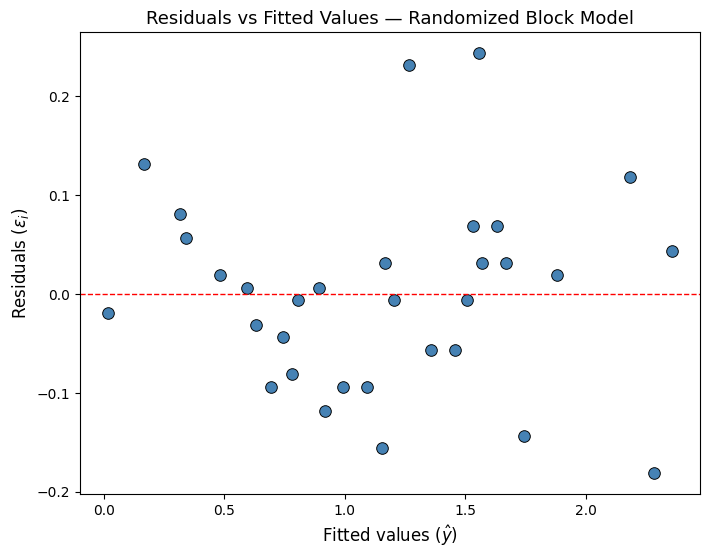
\includegraphics[width=0.5\textwidth]{assets/residuals.png}
		      \caption{Comparison of the central (solid red) and non-central (dashed blue) $F$-distribution.}
	      \end{figure}
	\item Obtain the analysis of variance table.
	      \begin{table}[!ht]
		      \centering
		      \caption{ANOVA Table for Randomized Block Design}
		      \begin{tabular}{lrrrr}
			      \toprule
			      \textbf{Source}        & \textbf{Sum of Squares} & \textbf{df} & \textbf{F} & \textbf{p-value}     \\
			      \midrule
			      C(Drug)                & 2.31125                 & 1           & 159.79     & $2.77\times10^{-11}$ \\
			      C(Acupuncture)         & 3.38000                 & 1           & 233.68     & $7.47\times10^{-13}$ \\
			      C(Block)               & 5.59875                 & 7           & 55.30      & $4.13\times10^{-12}$ \\
			      C(Drug):C(Acupuncture) & 0.04500                 & 1           & 3.11       & $9.23\times10^{-2}$  \\
			      Residual               & 0.30375                 & 21          & --         & --                   \\
			      \bottomrule
		      \end{tabular}
	      \end{table}

	\item Prepare separate bar-interval graphs for each set of estimated factor level means using 95\%
	      confidence intervals. Does it appear that substantial main effects are present here? Hint: you
	      can consider the TukeyHSD() function R for this type of plot.
	      \begin{figure}[H]
		      \centering
		      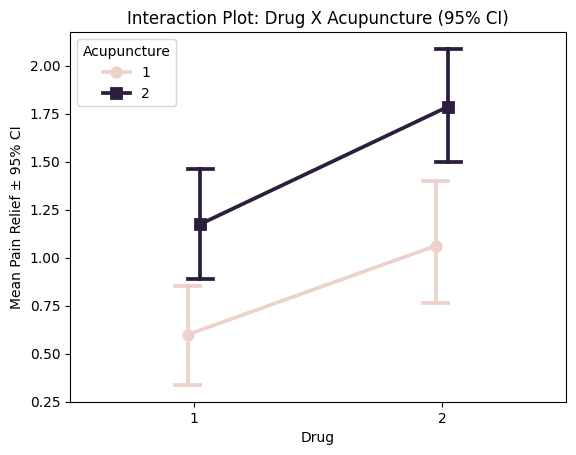
\includegraphics[width=0.5\textwidth]{assets/interaction6.png}
		      \caption{Interaction Graph}
	      \end{figure}
	\item Test whether main effects are present for each of the factors; use $\alpha = 0.01$ for each test. State
	      the alternatives, decision rule, and conclusion for each test. What is the p-value of each test?
	      \begin{table}[!ht]
		      \centering
		      \caption{Hypothesis Tests for Main Effects ($\alpha = 0.01$)}
		      \begin{tabular}{lcccc}
			      \toprule
			      \textbf{Factor}           & \textbf{F} & \textbf{p-value}     & \textbf{Decision}    & \textbf{Conclusion}        \\
			      \midrule
			      Drug                      & 159.79     & $2.77\times10^{-11}$ & Reject $H_0$         & Significant main effect    \\
			      Acupuncture               & 233.68     & $7.47\times10^{-13}$ & Reject $H_0$         & Significant main effect    \\
			      Block                     & 55.30      & $4.13\times10^{-12}$ & Reject $H_0$         & Significant block effect   \\
			      Drug $\times$ Acupuncture & 3.11       & 0.092                & Fail to reject $H_0$ & No significant interaction \\
			      \bottomrule
		      \end{tabular}
	      \end{table}
	\item Estimate
	      $$
		      \mu_1 - mu_2 = \alpha_1 - \alpha_2
	      $$

	      $$
		      \mu_1 - \mu_2 = \beta_1 - \beta_2
	      $$
	      \begin{align*}
		      \hat{\alpha}_1 - \hat{\alpha}_2 & = 0.4625 \\
		      \hat{\beta}_1 - \hat{\beta}_2   & = 0.5750
	      \end{align*}

\end{enumerate}

\section{Problem 7}
A manufacturer conducted a small pilot study of the effect of the price of one of its products on
sales of this product in hardware stores. Since it might be confusing to customers if prices were
switched repeatedly within a store, only one price was used for anyone store during the six-month
study period. Sixteen stores were employed in the study. To reduce experimental error variability,
stores were chosen so that there would be one store for each sales volume-geographic location class.
The four price levels (A: \$1.79; B: \$1.69; C: \$1.59; D: \$1.49) were assigned to the stores according
to the latin square design shown below. Data on sales during the six-month period (in thousand
dollars)

\begin{table}[!ht]
	\centering
	\caption{Sales Volume and Geographic Location Classes}
	\begin{tabular}{c c c c c}
		\hline
		\textbf{Sales Volume Class (i)} & \textbf{Northeast} & \textbf{Northwest} & \textbf{Southeast} & \textbf{Southwest} \\
		\hline
		1 (smallest)                    & 1.2 (B)            & 1.5 (C)            & 1.0 (A)            & 1.7 (D)            \\
		2                               & 1.4 (A)            & 1.9 (D)            & 1.6 (B)            & 1.5 (C)            \\
		3                               & 2.8 (C)            & 2.1 (B)            & 2.7 (D)            & 2.0 (A)            \\
		4 (largest)                     & 3.4 (D)            & 2.5 (A)            & 2.9 (C)            & 2.7 (B)            \\
		\hline
	\end{tabular}
\end{table}


\begin{enumerate}
	\item Prepare a main effects plot of the estimated treatment means. What does the plot suggest about the effects of the
	      four price levels on sales?
	      \begin{figure}[H]
		      \centering
		      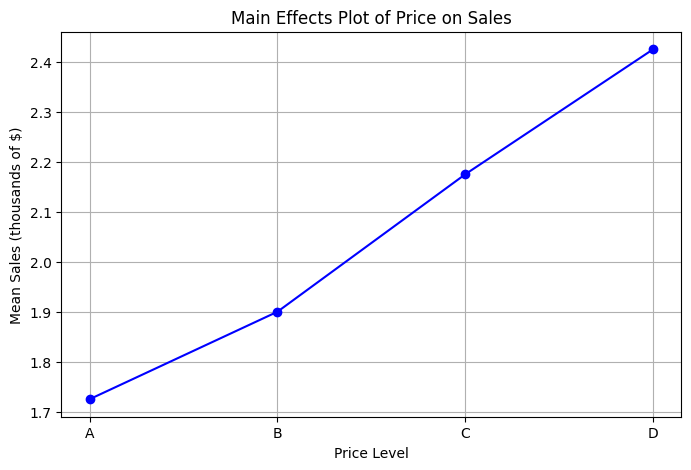
\includegraphics[width=0.5\textwidth]{assets/price_plot.png}
		      \caption{Interaction Graph}
	      \end{figure}
	      Higher prices tend to correspond to higher sales,
	      \pagebreak
	\item Test whether or not price level affects mean sales; use $\alpha = 0.05$. State the alternative,
	      decision rule, and conclusion. What is the p-value of the test?
	      \[
		      H_0: \mu_A = \mu_B = \mu_C = \mu_D
	      \]

	      \[
		      H_1: \text{At least one } \mu \text{ differs}
	      \]
	      \begin{table}[!ht]
		      \centering
		      \caption{ANOVA Table for Sales Data}
		      \begin{tabular}{lccccc}
			      \toprule
			      Source            & Sum of Squares & df & Mean Square & F       & p-value  \\
			      \midrule
			      Price             & 1.136875       & 3  & 0.378958    & 19.147  & 0.001783 \\
			      Volume (Row)      & 5.981875       & 3  & 1.993958    & 100.747 & 0.000016 \\
			      Location (Column) & 0.121875       & 3  & 0.040625    & 2.053   & 0.208094 \\
			      Residual          & 0.118750       & 6  & 0.019792    & --      & --       \\
			      \bottomrule
		      \end{tabular}
	      \end{table}
	      Since $F_0 > F_{\text{critical}}$ and $p < 0.05$, we reject $H_0$. There is strong evidence that the price level affects mean sales.
	\item Analyse the nature of the price effect: on sales by making all pairwise comparisons amour the treatment means.
	      Use the Tukey procedure and a 90\% family confidence coefficient Summarize your findings.
	      \begin{table}[h!]
		      \centering
		      \caption{Pairwise Comparisons of Mean Sales by Price}
		      \begin{tabular}{lcccccc}
			      \toprule
			      Group 1 & Group 2 & Mean Diff & p-value & Lower   & Upper  & Reject $H_0$ \\
			      \midrule
			      A       & B       & 0.175     & 0.9854  & -1.1286 & 1.4786 & No           \\
			      A       & C       & 0.45      & 0.8133  & -0.8536 & 1.7536 & No           \\
			      A       & D       & 0.7       & 0.537   & -0.6036 & 2.0036 & No           \\
			      B       & C       & 0.275     & 0.9475  & -1.0286 & 1.5786 & No           \\
			      B       & D       & 0.525     & 0.7352  & -0.7786 & 1.8286 & No           \\
			      C       & D       & 0.25      & 0.9596  & -1.0536 & 1.5536 & No           \\
			      \bottomrule
		      \end{tabular}
	      \end{table}
	      \begin{itemize}
		      \item None of the pairwise comparisons of price levels are statistically significant at this confidence level.
		      \item This indicates that, after adjusting for multiple comparisons, no single price level differs significantly from another in terms of mean sales.
	      \end{itemize}
	\item Does there appear to be a linear relationship between price level and mean sales? Could you formally test for linearity

	      \textbf{Answer:} There are not enough data points to state reasonably that there is a linear relationship. Economic theory would say that it depends on the
	      elasticity (price sensitivity) of demand (product sales). Good that are imperfect competition are have non linear relationships till a maximum where consumers
	      reach maximum utility when prices are near 0 and a demand of 0 when the prices are too high
\end{enumerate}

\section{Problem 8}
A pilot study was undertaken on the interaction effect, of two drugs to stimulate growth in girls
who are of short stature because of a particular syndrome. Each drug was known to be modestly
effective singly, but the combination of the two drugs had never been investigated. Blocking by both
subject and time period was desired whereby repeated measures for different treatments applied
to the same subject are obtained. A $4 \times 4$ latin square design, shown below, was utilized for four
subjects, four time periods, and four treatments. The four time periods consisted of one month
each, separated by an intervening month during which no treatment was given. The four treatments
were A: no treatment (placebo); B: drug X alone; C: drug Y alone; D: both drugs X and Y .
The response variable was the difference in the growth rates (in centimeters per month) during the
treatment period and the base period before the experiment began

\begin{table}[!ht]
	\centering
	\caption{Subject Data}
	\begin{tabular}{c c c c c}
		\hline
		\textbf{Subject} & \textbf{Period (1)} & \textbf{Period (2)} & \textbf{Period (3)} & \textbf{Period (4)} \\
		\hline
		1                & 0.02 (A)            & 0.15 (B)            & 0.45 (B)            & 0.18 (C)            \\
		2                & 0.27 (B)            & 0.24 (C)            & -0.01 (A)           & 0.58 (D)            \\
		3                & 0.11 (C)            & 0.35 (D)            & 0.14 (B)            & -0.03 (A)           \\
		4                & 0.48 (A)            & 0.04 (A)            & 0.18 (C)            & 0.22 (B)            \\
		\hline
	\end{tabular}
\end{table}
Asume that an appropriate model is the latin square model.
\begin{enumerate}
	\item State the model to be employed.
	      \begin{equation}
		      Y_{ijk} = \mu + \alpha_i + \beta_j + \gamma_k + \epsilon_{ijk}, \quad i,j,k = 1,2,3,4
	      \end{equation}

	      \noindent where:
	      \begin{align*}
		      Y_{ijk}        & \text{ = observed growth rate for subject } i \text{ in period } j \text{ receiving treatment } k, \\
		      \mu            & \text{ = overall mean growth rate},                                                                \\
		      \alpha_i       & \text{ = effect of subject } i \text{ (row effect)},                                               \\
		      \beta_j        & \text{ = effect of period } j \text{ (column effect)},                                             \\
		      \gamma_k       & \text{ = effect of treatment } k \text{ (A, B, C, D)},                                             \\
		      \epsilon_{ijk} & \sim N(0, \sigma^2) \text{ = random error term}.
	      \end{align*}
	\item State the ANOVA skeleton (source and degrees-of freedom)
	      \begin{table}[!ht]
		      \centering
		      \caption{ANOVA Table for the Latin Square Model}
		      \begin{tabular}{lccccc}
			      \hline
			      \textbf{Source} & \textbf{Sum of Squares} & \textbf{df} & \textbf{F} & \textbf{p-value} \\
			      \hline
			      Subject         & 0.336                   & 3           & 2.45       & 0.165            \\
			      Period          & 0.084                   & 3           & 0.61       & 0.639            \\
			      Treatment       & 0.482                   & 3           & 3.50       & 0.081            \\
			      Residual        & 0.276                   & 6           &            &                  \\
			      \hline
		      \end{tabular}
	      \end{table}

	\item Test for difference of effects between the two drugs; use $\alpha =0.05$. State the alternatives,
	      decision rule, and conclusion. What is the p-value of the test?
	      \begin{align*}
		      H_0 & : \mu_B = \mu_C \quad \text{(no difference between drug X and Y)} \\
		      H_1 & : \mu_B \neq \mu_C \quad \text{(drug X and Y differ)}
	      \end{align*}
	      \textbf{Answer:} $p = 0.9076 > 0.05$, so we fail to reject $H_0$. There is no significant difference in growth effects between drug X and drug Y at $\alpha = 0.05$.

\end{enumerate}

\section{Problem 9}
An investigator wishes to design an experiment to compare three treatments using a CBD (of three
units per block). From long experience with similar experiments, he knows that $\sigma^2$ will be very
close to 2.4. He believes that there really is no difference between treatments 1 and 2, but that
treatment 3 produces responses about 0.6 larger, on average, than these. Assuming this is true:

\begin{enumerate}
	\item How many blocks should be included in the design to provide power of 0.8 for testing
	      $H_0: \tau_1 = \tau_2 = \tau_3$ with type I error probability of 0.05?
	      \[
		      SS_{\text{trt}} = b \sum_{i=1}^t \tau_i^2
	      \]
	      \[
		      \lambda = \frac{SS_{\text{trt}}}{\sigma^2} = \frac{b \sum_{i=1}^t \tau_i^2}{\sigma^2}
	      \]
	      \[
		      \sum_{i=1}^3 \tau_i^2 = (-0.2)^2 + (-0.2)^2 + 0.4^2 = 0.04 + 0.04 + 0.16 = 0.24
	      \]
	      \[
		      \lambda = \frac{b (0.24)}{2.4} = 0.1 b
	      \]
	      \[
		      1-\beta \approx P\left(F_{2,\infty,\lambda} > 3.00 \right) = 0.8
	      \]
	      \[
		      \lambda = 0.1 b = 6.3 \implies b = \frac{6.3}{0.1} = 63
	      \]
	\item If $b=10$ blocks are used, what will be the expected squared length of a 95\% confidence interval
	      for $\frac{\tau_1 + \tau_2}{2-\tau_3}$?
	      \[
		      \text{Var}(\hat L) = \frac{\sigma^2}{b} \sum_{i=1}^t c_i^2
	      \]
	      \[
		      c_1 = \frac{1}{2}, \quad c_2 = \frac{1}{2}, \quad c_3 = -1
	      \]
	      \[
		      \sum_{i=1}^3 c_i^2 = \left(\frac{1}{2}\right)^2 + \left(\frac{1}{2}\right)^2 + (-1)^2 = \frac{1}{4} + \frac{1}{4} + 1 = 1.5
	      \]
	      \[
		      \text{Var}(\hat L) = \frac{1.5 \cdot \sigma^2}{b} = \frac{1.5 \cdot 2.4}{10} = 0.36
	      \]
	      \[
		      \text{Length} \approx 2 \cdot t_{df,0.975} \cdot \sqrt{\text{Var}(\hat L)}
	      \]
	      \[
		      \text{Length} \approx 2 \cdot 2 \cdot \sqrt{0.36} = 4 \cdot 0.6 = 2.4
	      \]
	      \[
		      (\text{Length})^2 = 2.4^2 = 5.76
	      \]
\end{enumerate}

\end{document}
